\chapter{Convolutional layers}
\label{chap:cnns}

\begin{supportbox}{About this chapter}
In this chapter we introduce our second core layer, the \textbf{convolutional layer}, which is designed to work with images (or, more in general, sequential data of any kind) by exploiting two  key ideas that we call \textit{locality} and \textit{parameter sharing}.
\end{supportbox}

Fully-connected layers are important historically, but less so from a practical point of view: on unstructured data (what we also call \textbf{tabular} data, as it can be easily represented as a table) MLPs are generally outperformed by other alternatives, such as random forests or well tuned support vector machines \cite{grinsztajn2022tree}. This is not true, however, as soon as we consider other types of data, having some structure that can be exploited in the design of the layers and of the model.

In this chapter we  consider the image domain, while in the next chapters we also consider applications to time series, audio, graphs, and videos. In all these cases, the input has a sequential structure (either temporal, spatial, or of other type) that can be leveraged to design layers that are both performant, easily composable, and highly efficient in terms of parameters. Interestingly, we will see that possible solutions can be designed by taking as starting point a fully-connected layer, and then suitably restricting or generalizing it based on the properties of the input.
%
\section{Towards convolutional layers}
\label{sec:towards_convolutive_layers}
%
\subsection{Why fully-connected layers are not enough}
%
An image can be described by a tensor $X \sim(h,w,c)$, where $h$ is the height of the image, $w$ the width of the image, and $c$ is the number of channels (which can be $1$ for black and white images, $3$ for color images, or higher for, e.g., hyper-spectral images). Hence, a mini-batch of images will generally be of rank $4$ with an additional leading batch dimension $(b, h, w, c)$. The three dimensions are not identical, since $h$ and $w$ represent a spatial arrangement of \textit{pixels}, while the channels $c$ do not have a specific ordering, in the sense that storing images in an RGB or a GBR format is only a matter of convention. 

\begin{supportbox}{On notation, channels, and features}
We use the same symbol we used for features in the tabular case ($c$) because it will play a similar role in the design of the models, i.e., we can think of each pixel as described by a generic set of $c$ \textit{features} which are updated in parallel by the layers of the model. Hence, the convolutional layer will return a generic tensor $(h,w,c^\prime)$ with an embedding of size $c^\prime$ for each of the $hw$ pixels.
\end{supportbox}

In order to use a fully-connected layer, we would need to “flatten” (vectorize) the image:
%
\begin{equation}
\mathbf{h} =\phi(\mathbf{W}\cdot \eqnmarkbox[drawred]{node}{\text{vect}(X)})
\label{eq:basic_image_layer}
\end{equation}
\annotate[yshift=-1em]{below,right}{node}{Flattened image}

\vspace{1em}
where $\text{vect}(x)$ is equivalent to {\footnotesize\mintinline{python}{x.reshape(-1)}} in PyTorch, and it returns for a generic rank-$n$ tensor $x \sim (i_1, i_2, \ldots, i_n)$ an equivalent tensor $\mathbf{x} \sim \left(\prod_{j=1}^n i_j\right)$.


Although it should be clear this is an inelegant approach, it is worth emphasizing some of its disadvantages. First, we have lost a very important property from the previous section, namely, \textbf{composability}: our input is an image, while our output is a vector, meaning we cannot concatenate two of these layers. We can recover this by reshaping the output vector to an image:
%
\begin{equation}
H = \text{unvect}(\phi(\mathbf{W}\cdot\text{vect}(X)))
\end{equation}
%
where we assume that the layer does not modify the number of pixels, and $\text{unvect}$ reshapes the output to a $(h,w,c^\prime)$ tensor, with $c^\prime$ an hyper-parameter. 

This leads directly to the second issue, which is that the layer has a \textit{huge} number of parameters. Considering, for example, a (1024, 1024) image in RGB, keeping the same dimensionality in output results in $(1024*1024*3)^2$ parameters (or $(hw)^2cc^\prime)$ in general), which is in the order of $10^{13}$! We can interpret the previous layer as follows: for each pixel, every channel in the output is a weighted combination of \textit{all} channels of \textit{all} pixels in the input image. As we will see, we can obtain a more efficient solution by restricting this computation.

\begin{supportbox}{More on reshaping}
%
In order to flatten (or more in general, reshape) a tensor, we need to decide an ordering in which to process the values. In practice, this is determined by the way the tensors are stored in memory: in most frameworks, the tensor's data is stored sequentially in a contiguous block of memory, in what is called a \textbf{strided layout}. Consider the following example:

\vspace{1em}
\begin{center}
\footnotesize
\mintinline{python}{torch.randn(32, 32, 3).stride() # [Out]: (96, 3, 1)}
\end{center}
\vspace{1em}

The stride is the number of steps that must be taken in memory to move of $1$ position along that axis, i.e., the last dimension of the tensor is contiguous, while to move of one position in the first dimension we need $96$ ($32*3$) steps. This is called a \textbf{row-major} ordering or, in image analysis, a \textbf{raster} order.\footnote{\url{https://en.wikipedia.org/wiki/Raster_scan}} Every reshaping operation works by moving along this strided representation.
%
\end{supportbox}

As a running example to visualize what follows, consider a 1D sequence (we will consider 1D sequences more in-depth later on; for now, you can think of this as “\textit{4 pixels with a single channel}”):

$$
\mathbf{x} = \left[x_1, x_2, x_3, x_4\right]
$$
%
In this case, we do not need any reshaping operations, and the previous layer (with $c^\prime = 1$) can be written as:
%
$$
\begin{bmatrix} h_1 \\ h_2 \\ h_3 \\ h_4 \end{bmatrix}=\begin{bmatrix}W_{11} & W_{12} & W_{13} & W_{14} \\ W_{21} & W_{22} & W_{23} & W_{24} \\ W_{31} & W_{32} & W_{33} & W_{34} \\ W_{41} & W_{42} & W_{43} & W_{44} \end{bmatrix} \begin{bmatrix} x_1 \\ x_2 \\ x_3 \\ x_4 \end{bmatrix}
$$

\begin{SCfigure}
    \centering
    \hspace{1em}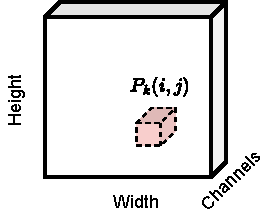
\includegraphics[width=0.4\textwidth]{images/patch}
    \caption{Given a tensor $(h,w,c)$ and a maximum distance $k$, the \textbf{patch} $P_k(i,j)$ (shown in red) is a $(2k+1,2k+1,c)$ tensor collecting all pixels at distance at most $k$ from the pixel in position $(i,j)$.}
    \label{fig:patch}
\end{SCfigure}

\subsection{Local layers}

The spatial arrangement of pixels introduces a metric (a distance) between the pixels. While there are many valid notions of “distance”, we will find it convenient to work with the following definition, which defines the distance between pixel $(i,j)$ and $(i^\prime, j^\prime)$ as the maximum distance across the two axes:
%
\begin{equation}
d((i,j), (i^\prime,j^\prime))=\max(\lvert i-i^\prime \rvert,\lvert j-j^\prime\rvert)
\label{eq:pixel_distance}
\end{equation}
%
How can we exploit this idea in the definition of a layer? Ideally, we can imagine that the influence of a pixel on another one decreases with a factor inversely proportional to their distance. Pushing this idea to its extreme, we can assume that the influence is effectively zero for a distance larger than some threshold. To formalize this insight, we introduce the concept of a \textbf{patch}.

\begin{definition}[Image patch] \addbottle
Given an image $X$, we define the \textbf{patch} $P_{k}(i,j)$ as the sub-image centered at $(i,j)$ and containing all pixels at distance equal or lower than $k$:
%
$$
P_{k}(i,j) = \idx{X}{i-k:i+k,j-k:j+k,:}
$$
%
where distance is defined as in \eqref{eq:pixel_distance}. This is shown visually in Figure \ref{fig:patch}.
%
\end{definition}



The definition is only valid for pixels which are at least $k$ steps away from the borders of the image: we will ignore this point for now and return to it later. Each patch is of shape $(s,s,c)$, where $s=2k+1$, since we consider $k$ pixels in each direction along with the central pixel. For reasons that will be clarified later on, we call $s$ the \textbf{filter size} or \textbf{kernel size}.

Consider a generic layer $H = f(X)$ taking as input a tensor of shape $(h,w,c)$ and returning a tensor of shape $(h,w,c^\prime)$. If the output for a given pixel only depends on a patch of predetermined size, we say that the layer is \textbf{local}.

\begin{definition}[Local layer]
Given an input image $X \sim(h,w,c)$, a layer $f(X) \sim(h,w,c^\prime)$ is \textbf{local} if there exists a $k$ such that:
%
$$
\idx{f(X)}{ij} = f(P_{k}(i, j))
$$
%
This has to hold for all pixels of the image.
%
\end{definition}

We can transform the layer \eqref{eq:basic_image_layer} into a local layer by setting to $0$ all weights belonging to pixels outside the influence region (\textbf{receptive field}) of each pixel:

\vspace{1em}
$$
H_{ij} =\phi\left(\eqnmarkbox[drawgreen]{node2}{\mathbf{W}_{ij}}\cdot\eqnmarkbox[drawred]{node}{\text{vect}(P_{k}(i,j))}\right)
$$
\annotate[yshift=1em]{above,right}{node}{Flattened patch (of shape $s^2c^\prime c$)}
\annotate[yshift=-1em]{below,right}{node2}{Position-dependent weight matrix}

\vspace{1em}
We call this class of layers \textbf{locally-connected}. Note that we have a different weight matrix $\mathbf{W}_{ij} \sim({c^\prime, ssc})$ for each output pixel, resulting in $hw(s^2cc^\prime)$ parameters. By comparison, we had $(hw)^2cc^\prime$ parameters in the initial layer, for a reduction factor of $\frac{s^2}{hw}$ in the number of parameters.

Considering our toy example, assuming for example $k=1$ (hence $s=3$) we can write the resulting operation as:
%
$$
\begin{bmatrix} h_1 \\ h_2 \\ h_3 \\ h_4 \end{bmatrix}=\begin{bmatrix}W_{12} & W_{13} & {\color{drawred}0} & {\color{drawred}0} \\ W_{21} & W_{22} & W_{23} & {\color{drawred}0} \\ {\color{drawred}0} & W_{31} & W_{32} & W_{33} \\ {\color{drawred}0} & {\color{drawred}0} & W_{41} & W_{42} \end{bmatrix} \begin{bmatrix} x_1 \\ x_2 \\ x_3 \\ x_4 \end{bmatrix}
$$
%
Our operation is not defined for $x_1$ and $x_4$, in which case we have considered a “shortened” filter by removing the weights corresponding to undefined operations. Equivalently, you can think of adding $0$ on the border whenever necessary:
%
$$
\begin{bmatrix} h_1 \\ h_2 \\ h_3 \\ h_4 \end{bmatrix}=\begin{bmatrix}W_{11} & W_{12} & W_{13} & 0 & 0 & {\color{drawred}0}\\ {\color{drawred}0} & W_{21} & W_{22} & W_{23} & 0 & {\color{drawred}0}\\ {\color{drawred}0} & 0 & W_{31} & W_{32} & W_{33} & {\color{drawred}0} \\ {\color{drawred}0} & 0 & 0 & W_{41} & W_{42} & W_{43} \end{bmatrix} \begin{bmatrix} {\color{drawred}0} \\ x_1 \\ x_2 \\ x_3 \\ x_4 \\ {\color{drawred}0} \end{bmatrix}
$$
%
This technique is called \textbf{zero-padding}. In an image, for a kernel size $2k+1$ we need exactly $k$ rows and columns of $0$ on each side to ensure that the operation is valid for each pixel. Otherwise, the output cannot be computed close to the borders, and the output tensor will have shape $(h-2k, w-2k, c^\prime)$. Both are valid options in most frameworks.

\begin{supportbox}{On our definition of patches}
The definition of convolutions using the idea of patches is a bit unconventional, but I find it to greatly simplify the notation. I provide a more conventional, signal processing oriented definition later on. The two definitions are equivalent and can be used interchangeably. The patch-oriented definition requires an \textbf{odd} kernel size and does not allow for \textbf{even} kernel sizes, but these are uncommon in practice.
\end{supportbox}

\subsection{Translation equivariance and the convolutive layer}

\addclock In a locally-connected layer, two identical patches can result in different outputs based on their location: some content on pixel $(5,2)$, for example, will be processed differently than the same content on pixel $(39, 81)$ because the two matrices $\mathbf{W}_{5,2}$ and $\mathbf{W}_{39,81}$ are different. For the most part, however, we can assume that this information is irrelevant: informally, “a horse is a horse”, irrespective of its positioning on the input image. We can formalize this with a property called \textbf{translation equivariance}.

\begin{definition}[Translation equivariance]
We say that a layer $H = f(X)$ is \textbf{translation equivariant} if:

$$
\eqnmarkbox[drawred]{node}{P_{k}(i,j) = P_{k}(i^\prime, j^\prime)} \;\; \textnormal{implies} \;\;  \eqnmarkbox[drawgreen]{node2}{f(P_{k}(i,j)) = f(P_{k}(i^\prime, j^\prime))}
$$
\annotate[yshift=-1em]{below,left}{node}{Identical patches}
\annotate[yshift=-1em]{below,right}{node2}{Identical outputs}

\end{definition}

\vspace{0.5em}
To understand the nomenclature, note that we can interpret the previous definition as follows: whenever an object moves (translates) on the image from position $(i,j)$ to position $(i^\prime, j^\prime)$, the output $f(P_{k}(i,j))$ that we we had in $(i,j)$ will now be found in $f(P_{k}(i^\prime,j^\prime))$. Hence, the activations of the layer are moving with the same (\textit{èqui} in Latin) translational movement as the input. We will define more formally equivariance and invariance later on.

A simple way to achieve translation equivariance is given by \textbf{weight sharing}, i.e., letting every position share the same set of weights:
%
$$
H_{ij} =\phi(\eqnmarkbox[drawred]{node}{\mathbf{W}}\cdot\text{vect}(P_{k}(i,j)))
$$
\annotate[yshift=-1em]{below,right}{node}{Weight matrix does not depend on $(i,j)$}

This is called a \textbf{convolutional layer}, and it is extremely efficient in terms of parameters: we only have a single weight matrix $\mathbf{W}$ of shape $(c^\prime, ssc)$, which is independent from the resolution of the original image (once again, contrast this with a layer which is only locally-connected with $hw(s^2c^\prime c)$ parameters: we have reduced them by another factor $\frac{1}{hw}$). We can write a variant with biases by adding $c^\prime$ additional parameters in the form of a bias vector $\mathbf{b} \sim (c^\prime)$. Because of its importance, we restate the full definition of the layer below.

\begin{definition}[Convolutional layer] \addbottle
%
Given an image $X \sim (h,w,c)$ and a kernel size $s=2k+1$, a \textbf{convolutional layer} $H=\textnormal{Conv2D}(X)$ is defined element-wise by:
%
\begin{equation}
H_{ij} = \mathbf{W} \cdot \textnormal{vect}(P_{k}(i,j)) + \mathbf{b}
\label{eq:convolutive_layer}
\end{equation}
%
The trainable parameters are $\mathbf{W} \sim (c^\prime, ssc)$ and $\mathbf{b} \sim (c^\prime)$. The hyper-parameters are $k$, $c^\prime$, and (eventually) whether to apply zero-padding or not. In the former case the output has shape $(h,w,c^\prime)$, in the latter case it has shape $(h-2k,w-2k,c^\prime)$. 
\end{definition}

\begin{mypy}{Convolution in PyTorch. Note that the channel dimension is -- by default -- the first one after the batch dimension. The kernel matrix is organized as a $(c^\prime, c, k, k)$ tensor. Padding can be specified as an integer or a string (`same' meaning that the output must have the same shape as the input, `valid' meaning no padding).}{code:convolution}
x = torch.randn(16, 3, 32, 32)
w = torch.randn(64, 3, 5, 5)
torch.nn.functional.conv2d(x, w, padding='same').shape 
# [Out]: torch.Size([16, 64, 32, 32])
\end{mypy}

See Box \ref{code:convolution} for a code example. The equivalent object-oriented implementation can be found in {\footnotesize\mintinline{python}{torch.nn.Conv2D}}. By comparison, our toy example can be refined as follows:

\begin{equation}
\begin{bmatrix} h_1 \\ h_2 \\ h_3 \\ h_4 \end{bmatrix}=\begin{bmatrix}{\color{drawred}W_2} & {\color{drawred}W_3} & 0 & 0 \\ {\color{drawred}W_1} & {\color{drawred}W_2} & {\color{drawred}W_3} & 0 \\ 0 & {\color{drawred}W_1} & {\color{drawred}W_2} & {\color{drawred}W_3} \\ 0 & 0 & {\color{drawred}W_1} & {\color{drawred}W_2} \end{bmatrix} \begin{bmatrix} x_1 \\ x_2 \\ x_3 \\ x_4 \end{bmatrix}
\label{eq:convolution_example}
\end{equation}

where we now have only three weights $\mathbf{W} = \left[W_1, W_2, W_3\right]^\top$ (the zero-padded version is equivalent to before and we omit it for brevity). This weight matrix has a special structure, where each element across any diagonal is a constant (e.g., on the main diagonal we only find $W_2$). We call these matrices \textbf{Toeplitz matrices},\footnote{\url{https://en.wikipedia.org/wiki/Toeplitz_matrix}} and they are fundamental to properly implement a convolutional layer on modern hardware. Toeplitz matrices are an example of \textbf{structured} dense matrices \cite{qiu2024compute}. Equation \eqref{eq:convolution_example} should also clarify that a convolution remains a \textit{linear} operation, albeit with a highly restricted weight matrix compared to a fully-connected one.

\subsection*{Convolutions and terminology}

\addteacup Our terminology comes (mostly) from signal processing. We can understand this by rewriting the output of the convolutional layer in a more standard form. To this end, we first rearrange the weight matrix into an equivalent weight tensor $W$ of shape $(s,s,c,c^\prime)$, similar to the PyTorch implementation in Box \ref{code:convolution}. For convenience, we also define a function that converts an integer $i^\prime$ from the interval $\left[1, \ldots, 2k+1\right]$ to the interval $\left[ i - k, \ldots, i + k\right]$:
%
\begin{equation}
t(i) = i - k - 1
\label{eq:convolutive_offset}
\end{equation}
%
where $k$ is left implicit in the arguments of $t(\bullet)$. We now rewrite the output of the layer with explicit summations across the axes:
%
\begin{equation}
H_{ijz} = \sum_{i^\prime=1}^{2k+1}\sum_{j^\prime = 1}^{2k+1}\sum_{d=1}^{c} \idx{W}{i^\prime, j^\prime, z, d}\idx{X}{i^\prime+t(i),j^\prime+t(j), d}
\label{eq:convolution_full_indexing}
\end{equation}
%
Check carefully the indexing: for a given pixel $(i,j)$ and output channel $z$ (a free index running from $1$ to $c^\prime$), on the spatial dimensions $W$ must be indexed along $1, 2, \ldots, 2k+1$, while $X$ must be indexed along $i-k, i-k+1, \ldots, i+k-1,i+k$. The index $d$ runs instead over the input channels.

From the point of view of signal processing, equation \eqref{eq:convolution_full_indexing} corresponds to a filtering operation on the input signal $X$ through a set of \textbf{finite impulse response} (FIR) filters \cite{uncini2015fundamentals}, implemented via a discrete convolution (apart from a sign change). Each filter here corresponds to a slice $W_{:,:,:,i}$ of the weight matrix. In standard signal processing, these filters can be manually designed to perform specific operations on the image. As an example, a $3 \times 3$ filter to detect ridges can be written as:\footnote{\url{https://en.wikipedia.org/wiki/Kernel_(image_processing)}}
%
$$
W =\begin{bmatrix}-1&-1&-1\\-1&8&-1\\-1&-1&-1\end{bmatrix}
$$
%
In convolutional layers, instead, these filters can be randomly initialized and trained via gradient descent. We consider the design of \textbf{convolutional models} built on convolutional layers in the next section. Before continuing, we mention that an interesting aspect of convolutional layers is that the output maintains a kind of “spatial consistency” and it can be plotted: we call a slice $H_{:,:,i}$ of the output an \textbf{activation map} of the layer, representing how much the specific filter was “activated” on each input region. We will consider in more detail the exploration of these maps in the next volume.

\section{Convolutional models}

\subsection{Designing convolutional “blocks”}

With the definition of a convolutional layer in hand, we now turn to the task of building \textbf{convolutional models}, also called \textbf{convolutional neural networks} (CNNs). We consider the problem of image classification, although a lot of what we say can be extended to other cases. To begin with, we formalize the concept of \textbf{receptive field}.

\begin{definition}[Receptive field]
Denote by $X$ an image, and by $H = g(X)$ a generic intermediate output of a convolutional model, e.g., the result of applying 1 or more convolutional layers. The \textbf{receptive field} $R(i,j)$ of pixel $(i,j)$ is the subset of $X$ which contributed to its computation:
$$
 \idx{g(X)}{ij} = g(R(i,j)), \;\;\; R(i,j) \subseteq X
$$
%
\end{definition}

For a single convolutional layer, the receptive field of a pixel is equal to a patch: $R(i,j) = P_{k}(i,j)$. However, it is easy to prove that for two convolutional layers in sequence with identical kernel size, the resulting receptive field is $R(i,j) = P_{2k}(i,j)$, then $P_{3k}(i,j)$ for three layers, and so on. Hence, the receptive field increases \textit{linearly} in the number of convolutional layers. This motivates our notion of locality: even if a single layer is limited in its receptive field by the kernel size, a sufficiently large stack of them results in a \textit{global} receptive field.

Consider now a sequence of two convolutional layers:
%
$$
H=\text{Conv}(\text{Conv}(X))
$$
%
Because convolution is a linear operation (see previous section), this is equivalent to a single convolution with a larger kernel size (as per the above). We can avoid this “collapse” in a similar way to fully-connected layers, by interleaving them with activation functions:
%
\begin{equation}
H = (\phi \circ \text{Conv}\circ\ldots\circ\phi\circ\text{Conv})(X)
\label{eq:convolutional_block}
\end{equation}
%
To continue with our design, we note that in \eqref{eq:convolutional_block} the channel dimension will be modified by each convolutional layer, while the spatial dimensions will remain of the same shape (or will be slightly reduced if we avoid zero-padding). However, it can be advantageous in practice to eventually reduce this dimensionality if our aim is something like image classification.

Consider again the example of a horse appearing in two different regions across two different images. The translation equivariance property of convolutional layers guarantees that every feature found in region 1 in the first image will be found, correspondingly, in region 2 of the second image. However, if our aim is “horse classification”, we eventually need one or more neurons activating for an horse \textit{irrespective of where it is found} in the image itself: if we only consider shifts, this property is called \textbf{translation invariance}.

Many operations that reduce over the spatial dimensions are trivially invariant to translations, for example:
%
$$
H^\prime=\sum_{i,j}H_{ij} \;\text{ or }\; H^\prime=\max_{i,j}(H_{ij})
$$
%
In the context of CNNs, this is called a \textbf{global pooling}. However, this destroys all spatial information present in the image. We can obtain a slightly more efficient solution with a partial reduction, called \textbf{max-pooling}. 

\begin{definition}[Max-pooling layer] \addbottle
Given a tensor $X \sim (h,w,c)$, a max-pooling layer, denoted as $\text{MaxPool(X)} \sim (\frac{h}{2}, \frac{w}{2}, c)$, is defined element-wise as:

$$
\idx{\textnormal{MaxPool}(X)}{ijc} = \max\left(\eqnmarkbox[drawred]{node}{\idx{X}{2i-1:2i, 2j-1:2j,c}}\right)
$$
\annotate[yshift=-1em]{below,right}{node}{$2 \times 2$ image patch}

\end{definition}

\vspace{1em}
Hence, we take $2\times 2$ windows of the input, and we compute the maximum value independently for each channel (this is generalized trivially to larger windows). Max-pooling effectively halves the spatial resolution while leaving the number of channels untouched. An example is shown in Figure \ref{fig:max_pooling}.

\begin{SCfigure}
    \centering
    \hspace{1em}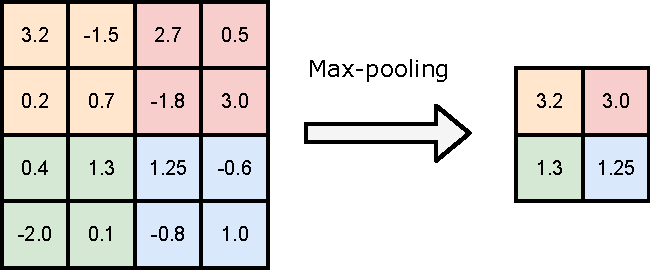
\includegraphics[width=0.5\textwidth]{images/max_pooling}
    \caption{Visualization of 2x2 max-pooling on a (4,4,1) image. For multiple channels, the operation is applied independently on each channel.
}
    \label{fig:max_pooling}
\end{SCfigure}

We can build a convolutional “block” by stacking several convolutional layers with a max-pooling operation  (see Figure \ref{fig:cnn_blocks}):
%
$$
\text{ConvBlock}(X)= (\text{MaxPool} \circ \phi \circ \text{Conv}\circ\ldots\circ\phi\circ\text{Conv})(X)
$$
%
And a more complex network by stacking together multiple such blocks:
%
\begin{equation}
H = (\text{ConvBlock}\circ\text{ConvBlock}\circ\ldots\circ\text{ConvBlock})(X)
\label{eq:convolutive_backbone}
\end{equation}
%
This design has a large number of hyper-parameters: the output channels of each layer, the kernel size of each layer, etc. It is common to drastically reduce the search space for the design by making some simplifying assumptions. For example, the VGG design \cite{szegedy2015going} popularized the idea of maintaining the filter size constant in each layer (e.g., $k=3$), while keeping the number of channels constant in each block and doubling them in-between every block.

\begin{SCfigure}
    \centering
    \hspace{1em}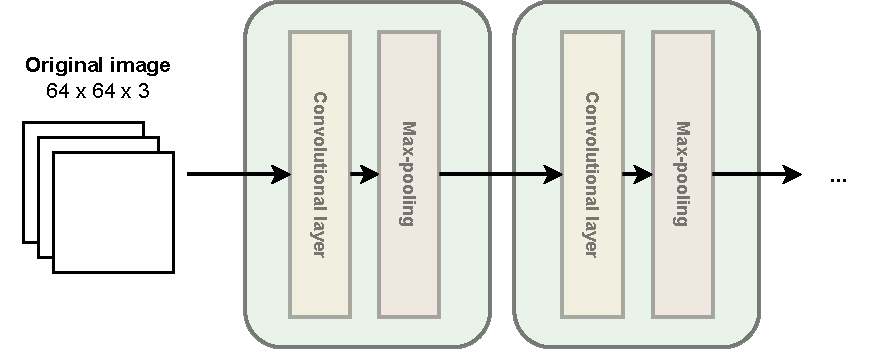
\includegraphics[width=0.6\textwidth]{images/CNN_blocks}
    \caption{Abstracting away from “layers” to “blocks” to simplify the design of differentiable models.}
    \label{fig:cnn_blocks}
\end{SCfigure}

An alternative way for reducing the dimensionality is to downsample the output of a convolutional layer: this is called the \textbf{stride} of the convolution. For example, a convolution with stride $1$ is a normal convolution, while a convolution with stride $2$ will compute only one output pixel every $2$, a convolution with stride $3$ will compute one output every $3$ pixels, and so on. Large strides and max-pooling can also be combined together depending on how the entire model is designed.

\begin{supportbox}{Invariance and equivariance}
Informally, if $T$ is a transformation on $x$ from some set (e.g., all possible shifts), we say a function $f$ is equivariant if $f(Tx)=Tf(x)$, and invariant if $f(Tx)=f(x)$. The space of all transformations form a group \cite{bronstein2017geometric}, and the matrix corresponding to a specific transformation is called a \textbf{representation} for that group. Convolutional layers are equivariant to translations by design, but other strategies can be found for more general forms of symmetries, such as averaging over the elements of the group (\textbf{frame averaging}, \cite{puny2021frame}). We will see other types of layers' equivariances in Chapter \ref{chap:gnns} and Chapter \ref{chap:transformers}.
\end{supportbox}

\subsection{Designing the complete model}

We can now complete the design of our model. By stacking together multiple convolutional blocks as in \eqref{eq:convolutive_backbone}, the output $H$ will be of shape $(h^\prime, w^\prime, c^\prime)$, where $w^\prime$ and $h^\prime$ depend on the number of max-pooling operations (or on the stride of the convolutional layers), while $c^\prime$ will depend only on the hyper-parameters of the last convolutional layer in the sequence. Note that each element $H_{ij}$ will correspond to a “macro-region” in the original image, e.g., if $h^\prime, w^\prime = 2$, $H_{11}$ will correspond to the “top-left” quadrant in the original image. We can remove this spatial dependency by performing a final global pooling operation before classification. 

The complete model, then, can be decomposed as three major components: a series of convolutional blocks, a global average pooling, and a final block for classification.
%
\begin{align} 
H = (\text{ConvBlock}\circ\ldots\circ\text{ConvBlock})(X) \label{eq:conv_blocks} \\
\mathbf{h}= \frac{1}{h^\prime w^\prime}\sum_{i,j}H_{ij}  \label{eq:global_avg_pooling} \\ 
y=\text{MLP}(\mathbf{h}) \label{eq:classification_head}
\end{align}
%
where $\text{MLP}(\mathbf{h})$ is a generic sequence of fully-connected layers (a flattening operation can also be used in place of the global pooling). This is a prototypical example of a CNN. See Figure \ref{fig:cnn_architecture} for a worked-out example.

\begin{figure}
    \centering
    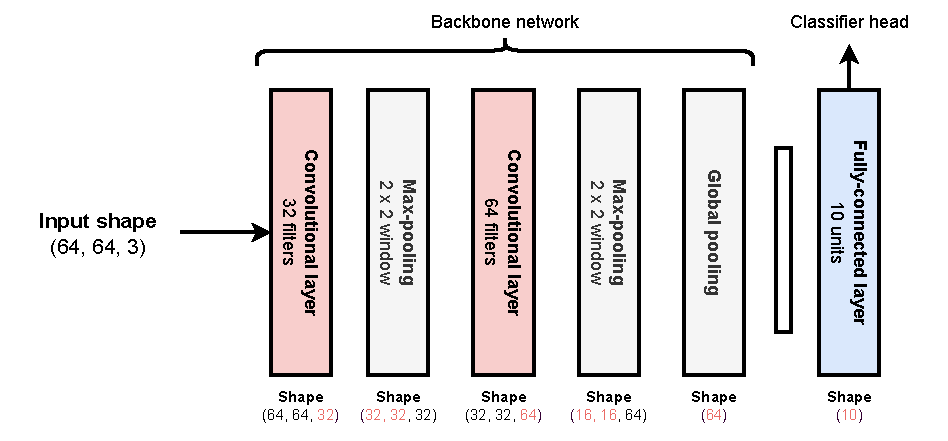
\includegraphics[width=0.9\textwidth]{images/CNN_architecture}
    \caption{Worked-out design of a very simple CNN for image classification (assuming 10 output classes). We show the output shape for each layer on the bottom. The global pooling operation can be replaced with a flattening operation. The last (\textbf{latent}) representation before the classification head is very useful when fine-tuning large-scale pre-trained models -- it is an \textbf{embedding} of the image in the sense of Section \ref{subsec:variants_supervised_learning}.}
    \label{fig:cnn_architecture}
\end{figure}

This design has a few interesting properties we list here:

\begin{enumerate}
\item It can be trained like the models described in Chapter \ref{chap:linear_models} and Chapter \ref{chap:fully_connected_models}. For example, for classification, we can wrap the output in a softmax and train by minimizing the cross-entropy. The same rules of back-propagation described in Chapter \ref{chap:automatic_differentiation} apply here.
\item Because of the global pooling operation, it does not depend on a specific input resolution. However, it is customary to fix this during training and inference to simplify mini-batching (more on variable length inputs in the next chapter).
\item \eqref{eq:global_avg_pooling} can be thought of as a “feature extraction” block, while \eqref{eq:classification_head} as the “classification block”. This interpretation will be very useful when we consider transfer learning in the next volume. We call the feature extraction block the \textbf{backbone} of the model, and the classification block the \textbf{head} of the model.
\end{enumerate}

\subsection*{Notable types of convolution}

We close the chapter by mentioning two instances of convolutional layers that are common in practice. 

First, consider a convolutional layer with $k=0$, i.e., a so-called $1 \times 1$ convolution. This corresponds to updating each pixel’s embedding by a weighted sum of its channels, disregarding all other pixels:
%
$$
H_{{\color{drawred}ij}z} = \sum_{t=1}^c W_{zt}X_{{\color{drawred}ij}t}
$$
%
It is a useful operation for, e.g., modifying the channel dimension (we will see an example when dealing with residual connections in Chapter \ref{chap:deep_cnns}). In this case, the parameters can be compactly represented by a matrix $\mathbf{W} \sim (c^\prime, c)$. This is equivalent to a fully-connected layer applied on each pixel independently.

Second, consider an “orthogonal” variant to $1 \times 1$ convolutions, in which we combine pixels in a small neighborhood, but disregarding all channels except one:
%
$$
H_{ij{\color{drawred}c}} = \sum_{i^\prime=1}^{2k+1}\sum_{j^\prime = 1}^{2k+1} W_{i^\prime, j^\prime,{\color{drawred}c}}X_{i^\prime +t(i),j^\prime+t(j),{\color{drawred}c}}
$$
%
where $t(\bullet)$ is the offset defined in \eqref{eq:convolutive_offset}. In this case we have a rank-$3$ weight matrix $W$ of shape $(s, s, c)$, and each output channel $H_{:,:,c}$ is updated by considering only the corresponding input channel $X_{:,:,c}$. This is called a \textbf{depthwise convolution}, and it can be generalized by considering groups of channels, in which case it is called a \textbf{groupwise convolution} (with the depthwise convolution being the extreme case of a group size equal to $1$).

We can also combine the two ideas and have a convolution block made of alternating $1 \times 1$ convolutions (to mix the channels) and depthwise convolutions (to mix the pixels). This is called a \textbf{depthwise separable} convolution and it is common in CNNs targeted for low-power devices \cite{howard2017mobilenets}. Note that in this case, the number of parameters for a single block (compared to a standard convolution) is reduced from $sscc^\prime$ to $ssc + cc^\prime$. We will see later how these decompositions, where the input is processed alternatively across separate axes, are fundamental for other types of architectures, such as transformers, in Chapter \ref{chap:transformers}.

\section*{From theory to practice}

\begin{wrapfigure}{r}{3.0cm}
\vspace{-3em}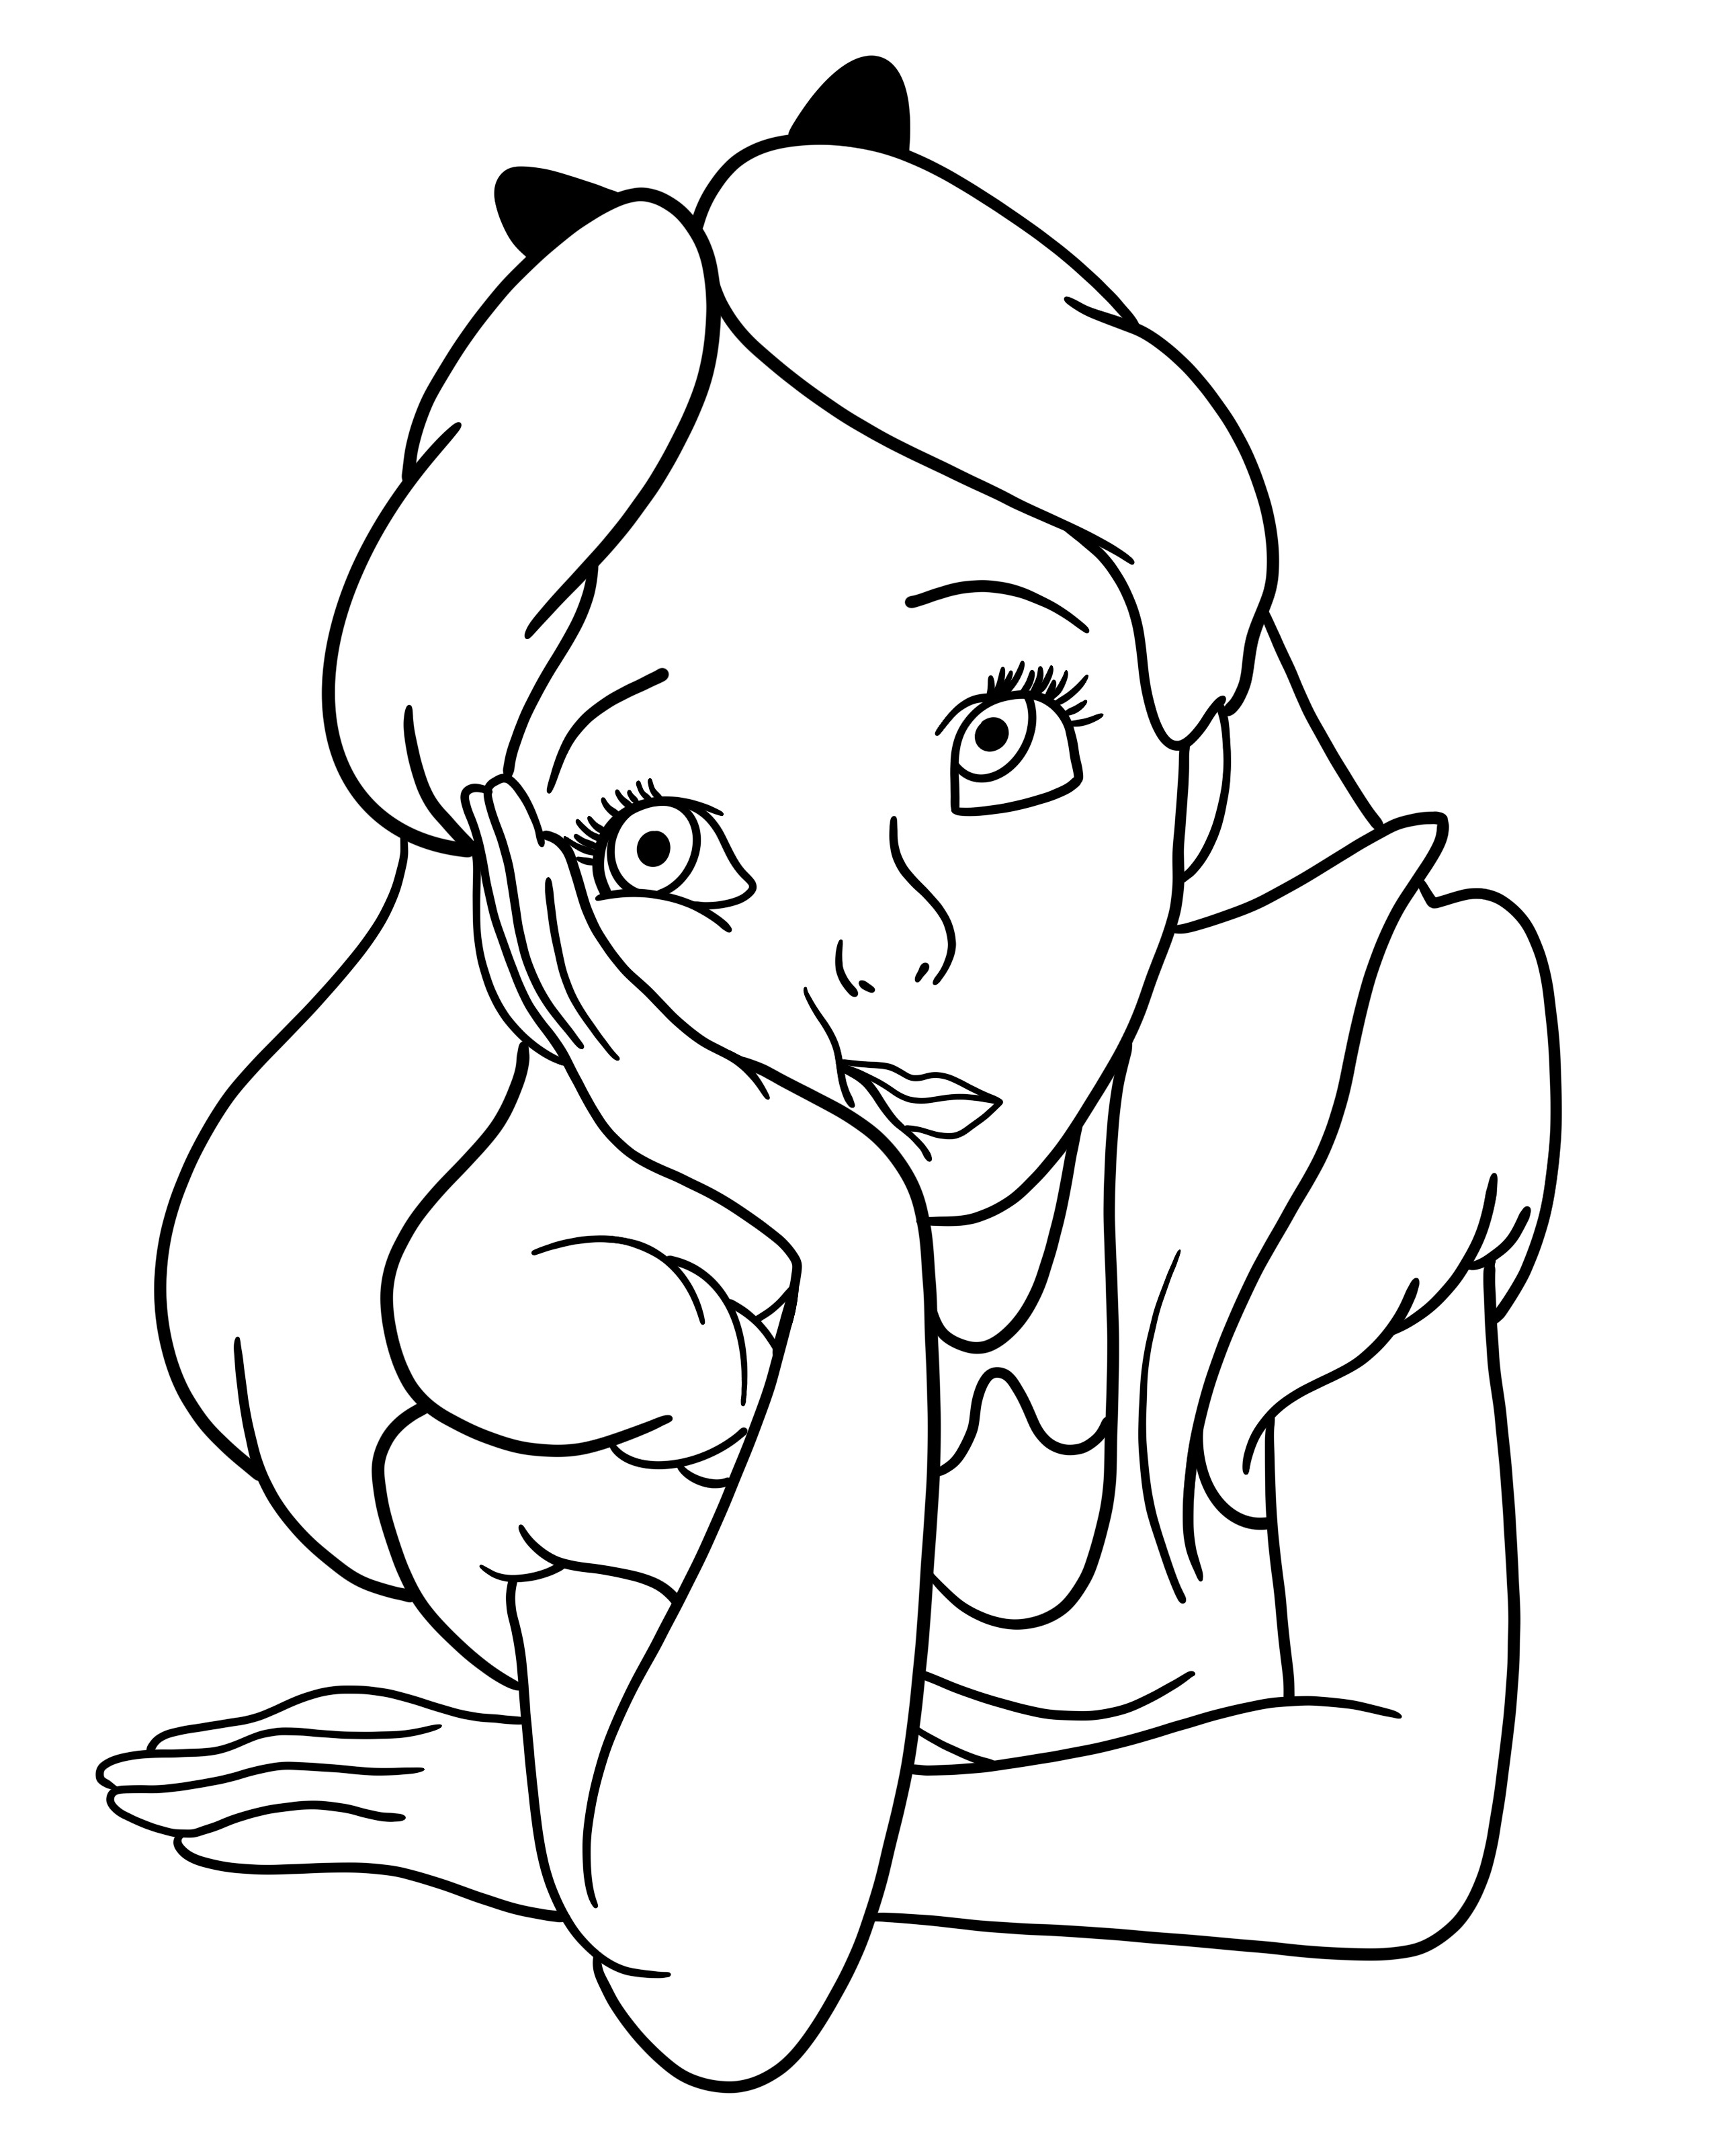
\includegraphics[width=3.0cm]{images/shutterstock_2075221579.jpg}
\vspace{-2em}
\end{wrapfigure}

All the layers introduced in this chapter (convolution, max-pooling) are implemented in the \mintinline{python}{torch.nn} module. The torchvision library provides datasets and functions to load images, as long as an interface to apply transformations to the images that will be very useful in the next chapter.\footnote{\url{https://pytorch.org/vision/stable/transforms.html}} 

Before proceeding, I suggest you follow and re-implement one of the many online tutorials on image classification in torchvision, which should now be relatively easy to follow.\footnote{As an example from the official documentation: \url{https://pytorch.org/tutorials/beginner/blitz/cifar10_tutorial.html}} Toy image datasets abound, including MNIST (digit classification) and CIFAR-10 (general image classification). Combining the torchvision loader with the layers in Equinox allows you to replicate the same tutorial in JAX, e.g., \url{https://docs.kidger.site/equinox/examples/mnist/}.

Implementing a convolution from scratch is also an interesting exercise, whose complexity depends on the level of abstraction. One possibility is to use the \texttt{fold}/\texttt{unfold} operations from PyTorch to extract the patches.\footnote{See for example: \url{https://github.com/loeweX/Custom-ConvLayers-Pytorch}} Premade kernels for convolutions will always be significantly faster, making this a purely didactic exercise.

If you have some signal processing background, you may know that convolution can also be implemented as multiplication by moving to the frequency domain. This is impractical for the small kernels used we tend to use, but it can be useful for very large (also known as \textit{long}) convolutions, e.g., \url{https://github.com/fkodom/fft-conv-pytorch}. PyTorch also provides a differentiable Fast Fourier transform that you can use as a starting point.